\section{Git operations}

\subsection{Add and Remove}

\subsubsection{What they do?}

When you use the 'git add <file>' command, a file will be
added to the index. The file added can be a new file, or 
a file already existing in the index. When the latter is true, 
git just updates the content of that file. \par
When you add a file, it will be marked to be committed in the next
commit. \par
'git rm <file>' can be seen as the inverse operation of the 'git add <file>'.
In this case Git, will remove a file from the index, so it won't appear in the
next commit. Besides being removed from index, it will also be removed from the 
working directory (if it's still there). \par

\subsubsection{Pre requisites}

There are a few cases where Git prevents you from removing a file : 
\begin{itemize}
\item The file must exist in the index.
\item Removing a file, when the file with it's current content 
doesn't exist in some commit object.
\end{itemize}
The last restriction exists, to avoid the accidental deletion of files. Imagine the
case where you have a file 'x' with 10k lines of code. You add it to the index,
but, before committing you accidentally use 'git rm x'. Because Git erases from
the index and the working directory you would lose it permanently.

\subsubsection{Properties}

\begin{itemize}
	\item Adding a file after adding the same file, has no effect
	\item Adding a file, committing, removing the same file and 
	committing brings to a commit equal to before of adding the file
	\item Removing a file and then adding the same file brings to an
	index equal to the one before removing the file
\end{itemize}

\subsubsection{Examples}

In these figures, it is shown the process of adding a file to the index. In
fact, both files showing represent the same file, but with different content at
a given time. So imagine that, after adding "File1", "File0" is added. "File1"
would be removed from the index (because there cannot be a file with different
contents in the index at any given state) and "File0" would be added. What was
described was the representation of the update of the content of a file in the
index. \par 
\begin{figure}[h!] 
	\caption{Before the add}
	\centering
	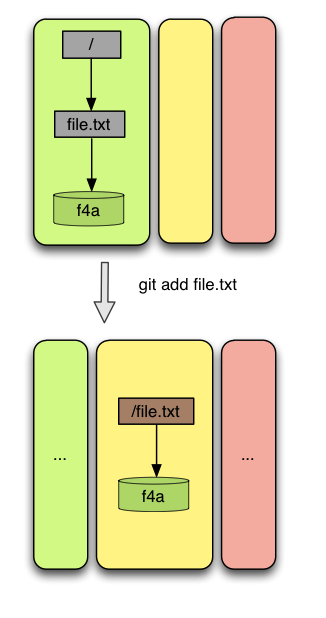
\includegraphics[scale=0.65]{images/add1.png}
\end{figure}

\begin{figure}[h!] 
	\caption{After the add}
	\centering
	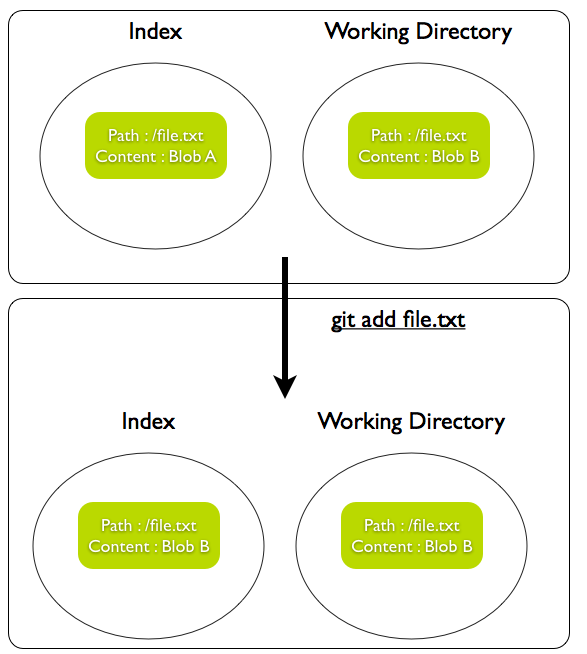
\includegraphics[scale=0.65]{images/add2.png}
\end{figure}

\pagebreak


\subsection{Commit}

\subsubsection{What it does?}

The 'git commit' operation, stores the current content of the index in a new
commit. \par
When the first commit is created, a branch called "Master" will be created
and will be marked as the current branch. Also, the first commit of a repository
is called a RootCommit. \par

\subsubsection{Pre requisites}

The only restriction that Git has about this operation 
it's that your new commit must have something different from the previous
commit, or, if it's the first commit, then there must exist some content in
current index. \par

\subsubsection{Properties}

\subsubsection{Examples}

\begin{figure} 
	\caption{A first commit}
	\centering
	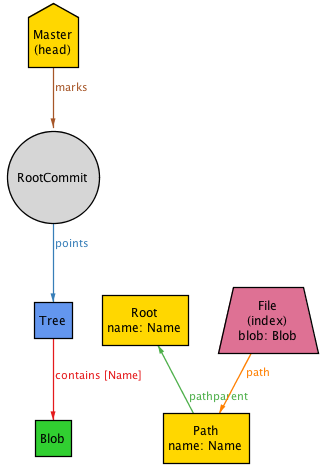
\includegraphics[scale=0.65]{images/commit1.png}
	\label{fig:commit1}
\end{figure}

The figure \ref{fig:commit1} is a typical example of a RootCommit. There is a file with the path
Name/Name, and a content Blob. It is currently on the index. The current branch
is Master, and it is pointing to a commit, which represents the index at current
state. \par

\begin{figure} 
	\caption{A Commit}
	\centering
	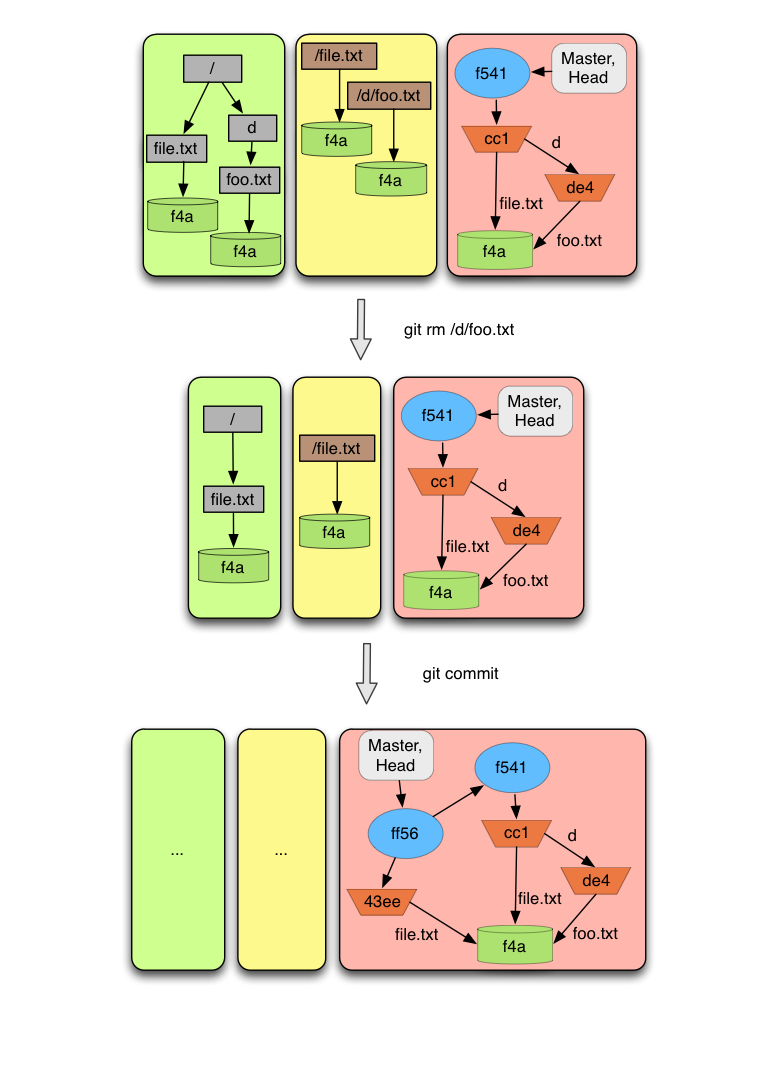
\includegraphics[scale=0.65]{images/commit2.png}
	\label{fig:commit2}
\end{figure}

The figure \ref{fig:commit2} represents the case of a normal commit, where the
newest commit comes after the RootCommit. The line of thought is the same as in
the last image. We can see that the difference between these two commits, it
that the only file was moved to a folder named "Name". \par
We can also see the efficiency of Git, about the sharing property of objects in
the commits, thus minimizing the space occupied in the repository. \par
\subsection{Branch}

\subsubsection{What it does?}
\subsubsection{Pre requisites}
\subsubsection{Properties}
\subsubsection{Examples}
Git branch operation has several forms, that to different things on git.
The ones which we care are the forms that create and delete branches. \par
When a new branch is created it will point to the current HEAD by default.
\par


The man git-branch says that when deleting a branch, it must be fully
merged in its upstream branch, or in HEAD if no upstream was set. \par


\subsection{Checkout}

\subsubsection{What it does?}
\subsubsection{Pre requisites}
\subsubsection{Properties}
\subsubsection{Examples}
From man git-checkout : "Switches branches by updating the index, 
working tree, and HEAD to reflect the specified branch or commit". \par

\subsection{Merge}

\subsubsection{What it does?}

When you do a 'git merge <branch>', a merge will happen between the current
branch and the branch selected on the command. The result will be a new merge 
commit, or a partially merged index. \par

Git knows three types of merge : 
\begin{itemize}
\item A fast-forward merge, that will happen when 
the current commit from the other
branch, is more recent than the current commit from the current branch. \par
This type is not a true merge, in the sense that the only thing that
changes it's the pointer of the current branch
is moved to the newest commit.

\item A 2-way merge, that happens when the conditions for a fast-forward
don't exist, and there isn't a common ancestor for both commits.

\item A 3-way merge, happens when the conditions for a fast-forward
don't exist, but, there is a common ancestor for both commits. \par
The difference between these two last types, is that the last is much 
more automatic having much less conflicts than the previous type.
\end{itemize}
Knowing these 3 types of merge, it's important to know that Git tries to make
the merge process as automatic as possible. However conflicts do exist, and when
they happen it leaves to the user the process of resolving those conflicts. \par
When the Git/user, finishes the merging of files in the index, he
can commit the resulting merge, in a merge commit. \par
Note that while there are unmerged files in the index, a commit cannot be
made. \par 

\subsubsection{Pre requisites}

\begin{itemize}
\item A merge can't be made, if the current commit is more recent then the
other commit.
\item A merge can't be made, while there are unmerged files.
\item In the case of a fast-forward merge, the index can't have uncommitted
files that can be changed by the merge operation.
\item In the case of a 2-way or 3-way merge operation there can not be
uncommitted files. 
\end{itemize}

\subsubsection{Properties}

\subsubsection{Examples}
